Money is a social construct, like trust. Both are very important and ephemeral things, and are being tested in a global digital world.  We are a long way from the village structures in which we evolved. We are now expected to casually adapt to the efficiencies promised by teams working in global mixed reality. This chaotic and intangible mix of value, trust, and socialisation is not well understood.\par
We wanted to explore exciting new developments in the transmission of value, and trust, in `digital society'. The problem is that each of these topics alone are enormously complex, and the intersections seem to be more so. We have been researching the current state-of-the-art, and the emerging consensus narrative, to try to figure out how the collision of these technologies might serve our virtual production workflows (Figure \ref{fig:pathway}).\par
Over the course of a couple of years the focus of the work has developed, and refined. The toolkit as it stands supports inclusive human creativity and economic exchange, especially for emerging markets and the global south. There is a huge proportion of human creativity currently excluded from media production pipelines due to gatekeepers of knowledge, access to identity proofs, and financial infrastructure that is taken for granted in the richer nations. This inclusion will be accomplished for the most part through integration of open source machine learning and AI tools, but this field quite new, and that part of the work is under developed.\par

\textbf{\hyperref[sec:tldr]{If at this stage you want to skip straight to the TL;DR for the whole book then click this bold text}.}\par
\begin{figure}
  \centering
   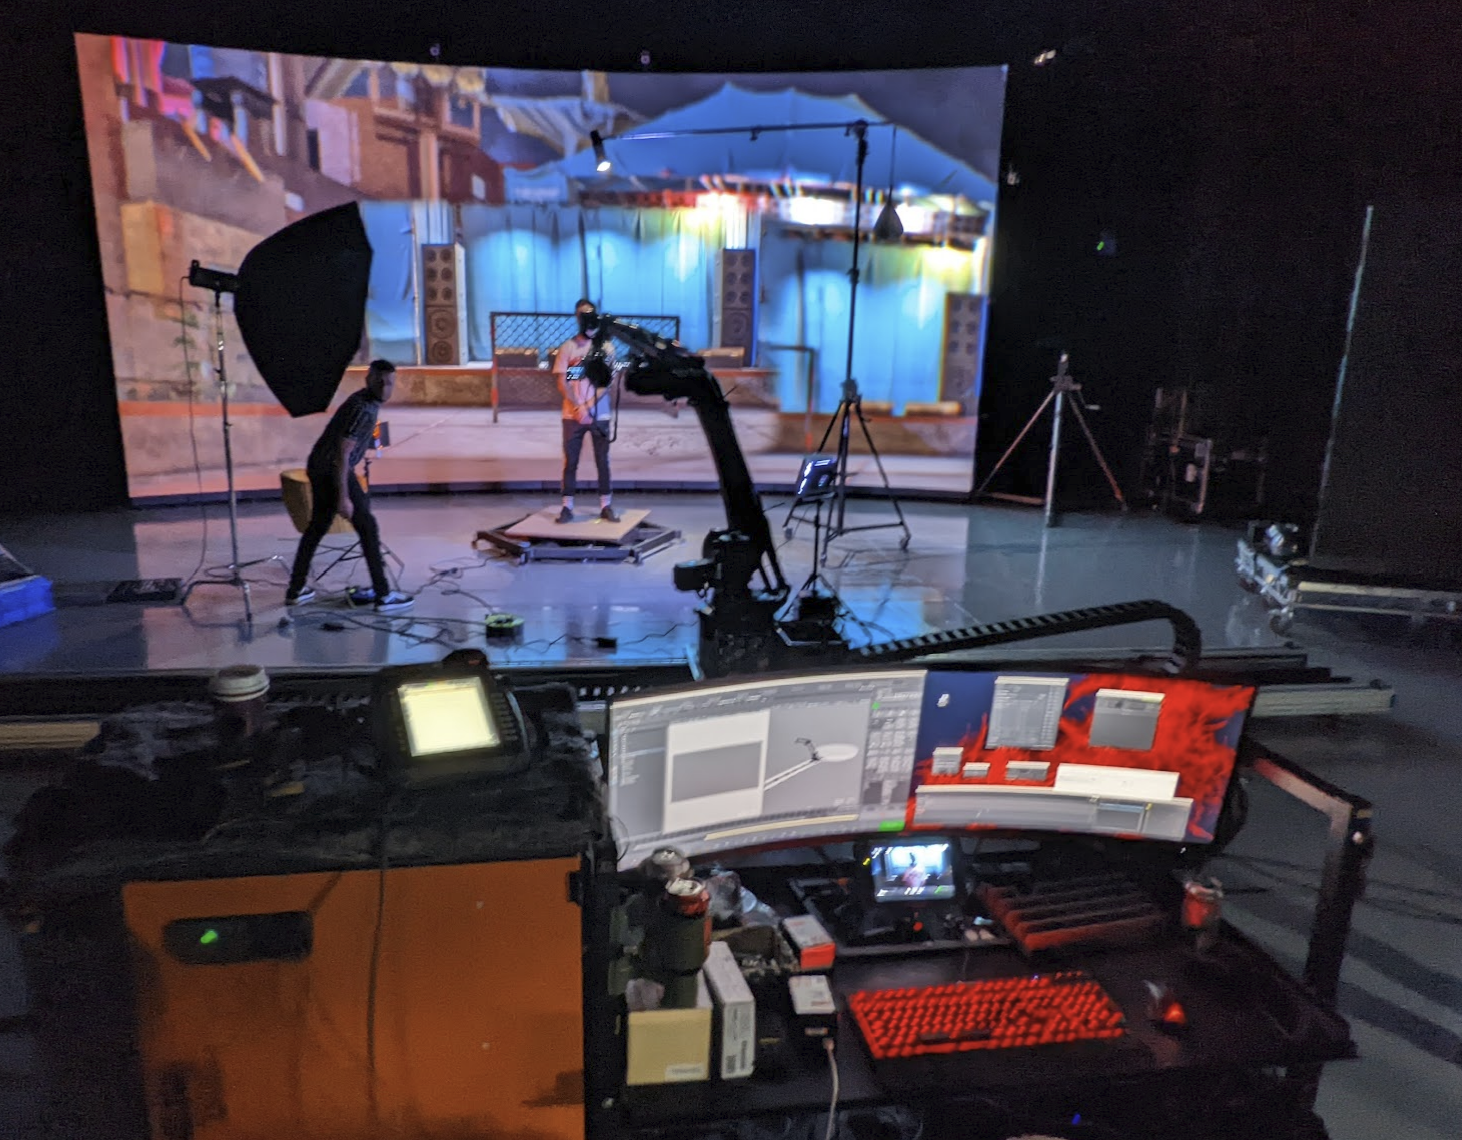
\includegraphics[width=\linewidth]{pathway}
 \caption{\href{https://www.pathwayxr.studio/}{Pathway XR virtual production}}
    \label{fig:pathway}
\end{figure}

